\documentclass[semcabeco,showtrims,trimframe,12pt,conselho,spreadimages]{memoir}

\usepackage[11x18]{hedraoptions} %% << %%%%%%%%%%%%%%%%
\usepackage[baruch]{hedrastyles}
\usepackage[xetex,chicagofootnotes]{tipografia}
\usepackage[standart,sempontinhos]{toc}
\usepackage{hedraextra}
\usepackage{penalidades}
\usepackage{graficos}
\usepackage{hedralogo}
\usepackage{hifensextras}
\usepackage{fichatecnica}
\usepackage[standart]{aparatos}
\usepackage{tabelas}
\usepackage{versos}
\usepackage{gitrevisioninfo}

\usepackage{wrapfig}

\newcommand{\forceindent}{\leavevmode{\parindent=1,4em\indent}}

\linespread{1.15}

\usepackage{endnotes}
\renewcommand{\notesname}{Notas}

%\counterwithin*{endnote}{part}
%\counterwithin*{endnote}{chapter}

\let\latexchapter\chapter
\makeatletter
\renewcommand\enoteheading{%
  \setcounter{secnumdepth}{-2}
  \latexchapter*{\notesname\markboth{NOTAS}{}}
  \mbox{}\par\vskip-\baselineskip
  \let\@afterindentfalse\@afterindenttrue
}
\makeatother
%\usepackage{fancyhdr}
%\pagestyle{fancy}
%\setlength{\headheight}{9mm}
%\fancyhf{}
%\fancyhead[R]{\thepage}
%\renewcommand{\headrulewidth}{0pt}

%\lhead[\fancyplain{}]{}
%\chead[\fancyplain{}]{}
%\rhead[\fancyplain{}]{\cnvt{\thepage} -- \thepage}

%\newcommand*{\cnvt}[1]{\the\numexpr#1-1\relax}

%\fancypagestyle{chapter}{
%\pagestyle{fancy}
%\setlength{\headheight}{5mm}
%\fancyhf{}
%\fancyhead[R]{\thepage}
%\renewcommand{\headrulewidth}{0pt}}

%--------------------------------------------PERMITIR FONTES MAIORES (HUGE)

\usepackage{anyfontsize}

%--------------------------------------------TIRAR TRAÇO DIVISOR DA FOOTNOTE

\usepackage{footmisc}

\renewcommand*\footnoterule{}
%\fancyhf[RO]{\cnvt{\thepage} -- \thepage}
%\fancyfoot{}
%\renewcommand{\headrulewidth}{0pt}
%\renewcommand{\footrulewidth}{0pt}}

%--------------------------------------------DEFININDO FONTES A SEREM USADAS NO LIVRO

\usepackage{fontspec}

\newcommand{\slsc}[1]{\fontspec[SmallCapsFeatures={FakeSlant=0.6}]{Formular-LightItalic}\textsc{#1}\fontspec[]{FormularLight-Italic}}

%\usepackage{Formular}
\newfontfamily\Formular{Formular-Regular}[
BoldFont = Formular-Bold.otf,
ItalicFont = Formular-Light.otf]
%\newfontfamily\Cobraarisca{Cobra arisca-Regular}
%\newfontfamily\fakereceipt{fake receipt}

%--------------------------------------------ALTERAR FONTE DA NOTA DE RODAPÉ

\setsansfont{Formular-Light}


\usepackage{etoolbox}
\makeatletter
\patchcmd{\@footnotetext}{\footnotesize}{\scriptsize\sffamily}{}{}
\makeatother

%--------------------------------------------ALTERAR FONTE DA NUMERAÇÃO DE PÁGINA
\usepackage{graphicx}
\usepackage{fancyhdr}
\pagestyle{fancy}
\fancyhf{}
\fancyfoot[CE,CO]{\Formular \footnotesize \textit \thepage}
\renewcommand{\headrulewidth}{0pt}

%--------------------------------------------ALTERAR DISTÃNCIA ENTRE TÍTULO DO SUMÁRIO E CAPÍTULOS
%\addtocontents{toc}{\vskip-15pt}
%--------------------------------------------
\usepackage{afterpage}

\newcommand\blankpage{%
    \null
    \thispagestyle{empty}%
    \addtocounter{page}{0}%
    \newpage}


\newenvironment{changemargin}[2]{%
\begin{list}{}{%
\setlength{\topsep}{0pt}%
\setlength{\leftmargin}{#1}%
\setlength{\rightmargin}{#2}%
\setlength{\listparindent}{\parindent}%
\setlength{\itemindent}{\parindent}%
\setlength{\parsep}{\parskip}%
}%
\item[]}{\end{list}}



\usepackage{changepage}
\usepackage{placeins}
\usepackage{float}
\usepackage{floatpag}
\usepackage{rotating}
%\usepackage{afterpage}
\usepackage{paracol}
\setlength{\columnsep}{0.8cm}

\newenvironment{absolutelynopagebreak}
  {\par\nobreak\vfil\penalty0\vfilneg
   \vtop\bgroup}
  {\par\xdef\tpd{\the\prevdepth}\egroup
   \prevdepth=\tpd}

%\usepackage{imakeidx} 
%\makeindex[program=xindy, options=-C utf8 -L portuguese]
%\newcommand\gobbleone[1]{}
%\newcommand*{\seeonly}[2]{\ (\emph{\seename} #1)}
%\newcommand*{\also}[2]{\emph{cf.} #1}
%\newcommand{\Also}[2]{\emph{See also} #1}
%\renewcommand\indexname{Índice onomástico}
%\makeindex[intoc]

\setcounter{tocdepth}{1}
\setcounter{secnumdepth}{-2} 
%\linespread{1.08}

\makeatletter
\newenvironment{Parskip}{%
   \par
   \parskip=0.3\baselineskip \advance\parskip by 0pt plus 2pt
   \parindent=\z@
   \def\@listI{\leftmargin\leftmargini
      \topsep\z@ \parsep\parskip \itemsep\z@}
   \let\@listi\@listI
   \@listi
   \def\@listii{\leftmargin\leftmarginii
      \labelwidth\leftmarginii\advance\labelwidth-\labelsep
      \topsep\z@ \parsep\parskip \itemsep\z@}
   \def\@listiii{\leftmargin\leftmarginiii
       \labelwidth\leftmarginiii\advance\labelwidth-\labelsep
       \topsep\z@ \parsep\parskip \itemsep\z@}
   \partopsep=\z@
}{\par}
\makeatother

\makeatletter
\newenvironment{myParskip}{%
   \par
   \parskip=0.2\baselineskip \advance\parskip by 0pt plus 2pt
   \parindent=\z@
   \def\@listI{\leftmargin\leftmargini
      \topsep\z@ \parsep\parskip \itemsep\z@}
   \let\@listi\@listI
   \@listi
   \def\@listii{\leftmargin\leftmarginii
      \labelwidth\leftmarginii\advance\labelwidth-\labelsep
      \topsep\z@ \parsep\parskip \itemsep\z@}
   \def\@listiii{\leftmargin\leftmarginiii
       \labelwidth\leftmarginiii\advance\labelwidth-\labelsep
       \topsep\z@ \parsep\parskip \itemsep\z@}
   \partopsep=\z@
}{\par}
\makeatother

\newcommand{\mystar}{{\fontfamily{lmr}\selectfont$\star$}}

%\makeatletter
%\renewcommand{\@chapapp}{}% Not necessary...
%\newenvironment{chapquote}[2][2em]
%  {\setlength{\@tempdima}{#1}%
%   \def\chapquote@author{#2}%
%   \parshape 1 \@tempdima \dimexpr\textwidth-2\@tempdima\relax%
%   \itshape}
%  {\par\scriptsize\hfill-- \chapquote@author\hspace*{\@tempdima}\par\bigskip}
%\makeatother

%\newcommand\Chapter[2]{\chapter
%  [#1\hfil\hbox{}\protect\linebreak{\itshape#1}]%
%  {#1\\[2ex]\Large\itshape#2}%
%}

\begin{document}

\pagebreak
\thispagestyle{empty}
\movetooddpage
\thispagestyle{empty}
\begin{vplace}[0.25]


{\large\Formular{
\noindent{}Prefácio publicado com\\ a reedição de 1960}}
\end{vplace}

\pagebreak
\thispagestyle{empty}

\movetooddpage

Este livrinho foi escrito em 1943, editado em 1945. Dez anos depois, me
falaram para fazer uma nova edição. Eu o reli. Indignado, comecei a
preparar uma crítica rigorosa daquelas pequenas fórmulas sob o título:
\emph{Semente de crápula ou o charlatão de boa vontade}. Essa
autocrítica, relida hoje, no inverno das Cévennes, me parece bem
excessiva, agressiva, peremptória. Ela ficará no caixa de madeira no
qual se amontoam, a cada mudança, páginas e páginas de intenções e
relatos que, talvez, sejam para mim o que as folhas que caem são para as
árvores.

No entanto, me incomoda deixar que saiam novos exemplares de
\emph{Semente de crápula} sem dizer nada. Tenho quinze ou dezesseis anos
a mais, quinze ou dezesseis anos nesse trabalho diário do qual eu falava
alegremente em 1943.

Palavras me vêm, páginas, capítulos, se me deixo levar.

Este livrinho precisa de um subtítulo que me situe, agora, em relação ao
que escrevi há quinze anos. Tenho este subtítulo: \emph{Semente de
crápula ou o amador de pipas}.

Era uma vez um amador de pipas. Vocês já sabem o que é uma pipa em
relação às nuvens, aos pássaros, aos aviões e satélites; ela não é
encontrada na natureza, é possível fazê"-la por si mesmo a partir de
modelos propostos em revistas ou folhetos, ou ainda inventar novas
formas inspiradas em pipas chinesas ancestrais, no abutre dos Andes ou
no avião"-caça Mystère \versal{IV}. Uma pipa não atravessa os muros do espaço, não
troveja nem zune, falta um não"-sei"-quê para que ela se sustente no vento
e continue alegrando, com um ponto de cor viva, o mais cinza dos céus,
ou para que ela caia e, pelo menos, não quebre nada além de sua própria
armação. À primeira vista, isso não serve para nada. Veremos.

Então, por volta de 1943, comecei a fazer uma pipa, duas pipas: as
fórmulas, formulinhas, cantigas, charadas, aforismos e paradoxos de
\emph{Semente de crápula}.

Uma pipa, sobretudo se for pequena, é fácil de segurar. Cento e trinta e
seis já é outro assunto: elas arrastam você, ainda que tenha pouco
vento, levantariam você, não podemos dizer que acima de você mesmo e,
contudo, acabei sendo um educador de renome, levado, pela força e pela
graça dessas cento e trinta e seis pequenas pipas, a um congresso
internacional aqui, a uma comissão ali, e por mais que eu puxasse as
cordas, como fazem os mergulhadores quando querem voltar a subir, minhas
pipas frequentemente me deixaram mofando ali, de onde eu teria querido
escapar.

Aconteceram"-me coisas piores. Sempre provocado por esse rebanho de
discursos díspares em cuja forma eu mesmo havia mexido à vontade,
encontrei"-me à frente na criação de organismos de reeducação. Pobre de
mim: aí é que se enredam os discursos e seus fios. É aí que o pobre
diabo que segura com a mão direita seu ramo de pequenas bandeiras
multiformes e multicolores se dá conta de que só lhe resta uma das mãos,
a outra, para lutar a todo custo, sem muralha nem certeza para se
apoiar. Com sorte, uma ou outra dessas fórmulas, soltas há muito tempo,
não acaba caindo sobre sua cabeça e seus ombros, cegando"-o, envolvendo"-o
com as tiras de sua rabiola, sobre as quais algumas palavras estão
escritas e ele desprega uma por acaso e a aplica e diz uma palavra em
falso como se faz um movimento em falso.

É isso provavelmente o que eu queria contar aos antigos e futuros
leitores de \emph{Semente de crápula}. Há dois mundos. Aquele das
fórmulas, formulinhas, charadas e parábolas e aquele do que acontece a
todo momento aqui embaixo com quem quer ajudar os outros. Se, uma vez
lidas, algumas de minhas palavras estremecem alegremente no céu de
algumas memórias, melhor assim: aí está sua razão de ser. Mas aquele que
quiser se servir delas, aplicá"-las de alguma maneira, se daria conta, ao
mesmo tempo, do que são feitas: pedaços de páginas lidas, coladas e
penduradas sobre os galhos maleáveis e leves arrancados de uma espécie
particular de entusiasmo que surge cada vez que um menino me aborda. Que
foi mil vezes serrado, derrubado e de cujo tronco nunca param de brotar
rebentos.

\hfill{}Fernand Deligny

\hfill{}janeiro de 1960

\pagebreak
\movetooddpage
\thispagestyle{empty}
\begin{vplace}[.25]


{\large\Formular{
\noindent{}Semente de crápula:\\ conselhos aos educadores\\ que queiram cultivá-la}}
\end{vplace}

\begin{center}
\vspace*{-4cm}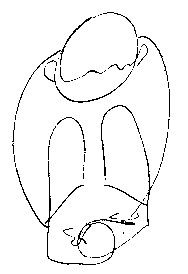
\includegraphics[width=.5\textwidth]{./imgs/Image_1.jpg}{}
\end{center}

\vspace{2cm}
{\Formular{\noindent{}Juliana Jardim\\ Luiz Pimentel\\ ({\slsc{tradução}})
}}

\pagebreak
\thispagestyle{empty}
\flushbottom

\movetooddpage


\letra{S}{e} você convive com filhotes de homem numa escola, num reformatório,
numa colônia de férias, já conhece a semente de crápula, tal como o
cultivador conhece o cardo, o joio, a papoula ou a nigela,
amaldiçoando"-os. Suponha agora que você, curioso cultivador, tenha
semeado um campo de joio, de cardo, de nigela ou de papoula. Ao vê"-los
sair da terra, você sentirá as mesmas angústias que experimentava ao ver
seu trigo germinar. Mas não se apresse em varrer os celeiros, nem
prepare já as cordas de colheita. A colheita, se colheita houver, será
para daqui a pouco, para mais tarde ou nunca. Com a diferença de que a
semente de crápula é, ainda assim, a semente de homem.


\letra{J}{á} que todos sabem que você cultiva o cardo, o joio, a papoula e a
nigela, espere para ver chegarem os cultivadores, de tamancos, bem à
vontade, olhando seu campo e dizendo: ``Eis a nigela, o joio, a papoula
e o cardo que infectam nossos campos,cuidados como ninguém sequer
pensaria em cuidar do trigo''. Se gosta que riam um pouco às suas
custas, responda, com os olhos para o céu e as mãos abertas: ``Sim, e
acredito que a colheita será linda''. Mas já se sabe que a semente de
crápula é, ainda assim, a semente de homem. Ou então, você seria mesmo
tão louco quanto parece. \enlargethispage{\baselineskip}

\pagebreak

\letra{E}{ste} aqui grita e gesticula, lhe aborda com projetos e reclamações;
aquele ali dorme, e dorme sem sonhos. Você pensa: ``A tarefa é fácil;
vou despertar o dorminhoco e acalmar o agitado''. Mas não consegue,
porque é impossível, porque a planta está na semente e a semente já é
planta. Para o agitado, ache um trabalho que ocupará utilmente sua
agitação e ensine o dorminhoco a trabalhar dormindo. Ao fazer isso, você
não será tão forte quanto o bom Deus, mas terá feito o seu possível.



\letra{E}{,} por favor, não conte com o poder das palavras. Você já ouviu alguma
vez um camponês conversar com suas beterrabas, um verdureiro com suas
folhas, um viticultor com suas uvas? Eles fazem o que é preciso para que
as plantas cresçam, e são muito respeitosos com o tempo. Não estou
falando para você da chuva e do vento, mas da duração necessária para
que as coisas se realizem. Quando resmungam ``isso não vai dar certo'',
é porque não há nada mais a ser feito. E se você me disser: ``É, mas os
filhotes de homem têm orelhas'', eu responderei: ``Infelizmente\ldots{} se
esse buraco não existisse, os adultos não poderiam despejar nele suas
idiotices''.


%\begin{wrapfigure}{r}{3cm}
 % 
\includegraphics[width=40mm]{./imgs/Image_2.jpg}
 %\end{wrapfigure}
\pagebreak
\thispagestyle{empty}

\begin{vplace}[1]
\begin{center}

\includegraphics[width=45mm]{./imgs/Image_2.jpg}
\end{center}
\end{vplace}

\pagebreak
\thispagestyle{empty}

\movetooddpage
%\flushbottom

\letra{V}{ocê,} com seus botões: ``Eles roubaram, fugiram de casa e vagabundearam:
errantes como lobos, sorrateiros como animais selvagens\ldots{} Por via das
dúvidas, vou abrir o peito e fazer, mandíbulas cerradas, um olhar de
domador\ldots{}'' E você os encontra servis, aduladores, solícitos e
obedientes. Oferecem"-lhe, já que é só o que podem dar, suas mãos, seus
sorrisos e seus ouvidos. Você pensa: ``Eu os conquistei''. Os dois furos
nos pneus da sua bicicleta são para completar o presente, aquele dom
próprio deles, e que provavelmente julgavam ser insuficiente.




\letra{R}{ejeite} os que vêm se oferecer: não vá procurar os que se afastam de
você, e conte os que ficam. Se só tiver um, comece com esse.




\letra{V}{ocê} é severo demais? Eles vão se esconder. Não é severo o bastante?
Então não vai impedi"-los de fazer bobagem. Não se preocupe, portanto,
com a severidade.




%\begin{center}
%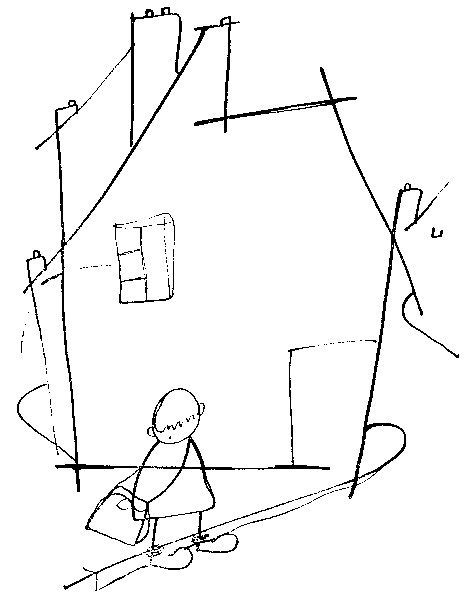
\includegraphics[width=70mm]{./imgs/Image_3.jpg}
%\end{center}

\pagebreak

\letra{V}{ocê,} com seus botões: ``Cuidado! trata"-se de uma luta. Uma vontade -- a
minha -- contra cem vontades hostis -- as deles''. E você se prepara e
se excita e perde seu tempo: vontade eles não têm. O que você precisa
fazer é ir lá para a frente e puxar, puxá"-los rumo a um objetivo. E pode
se segurar, pois isso é pesado e escorrega. Durante esse tempo, enquanto
você estiver bem ocupado apressando"-os na direção da luz e do sol, eles
vão surrupiar peras nos pomares vizinhos. É preciso, pois, se posicionar
atrás deles, para vigiá"-los. Não tendo mais ninguém para seguir, eles se
dispersam. E você volta para casa, bastante enojado do seu novo ofício
de pastor.



\letra{H.}{} foi posto no mundo pela mãe, criado pela tia, depois por uma prima,
puseram"-no numa fazenda, os avós tiraram"-no de lá, até chegar a você,
recém"-saído da prisão. E você acusa a sociedade? Quando conhecer H.,
você estará cheio de indulgência pela mãe, pela tia, pela prima, pelo
fazendeiro, pelo avô e pelo diretor da prisão. Isso não tira a culpa da
sociedade.



\letra{P}{equenos} azarados? Veremos. Deixe que as boas almas caridosas façam
cócegas no sentimentalismo. Você, faça seu trabalho.


\pagebreak
\thispagestyle{empty}

\begin{vplace}[.50]
\begin{center}
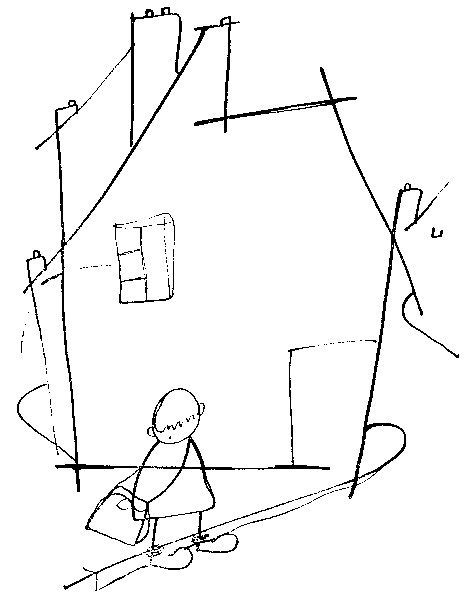
\includegraphics[width=95mm]{./imgs/Image_3.jpg}
\end{center}
\end{vplace}

\pagebreak
\thispagestyle{empty}


\movetooddpage

\letra{E}{les} conhecem todos os métodos de sedução, da mão no ombro até o pontapé
em qualquer lugar, passando pelo sermão com voz contida, olhos nos
olhos. Pelo efeito que isso já teve neles, tente outra coisa.




\letra{É}{} preciso saber o que você quer. Se quer que gostem de você, traga
balas. Mas o dia em que vier de mãos vazias, vão lhe chamar de escroto.
Se quiser fazer seu trabalho, dê"-lhes uma corda para puxar, madeira para
quebrar, sacos para carregar. O amor virá em seguida, e essa não é a sua
recompensa.




\letra{S}{e} você chega com os bolsos cheios de brinquedos, em uma hora eles os
transformarão em madeira quebrada. Se chega com a cabeça cheia de
projetos, em três dias eles estarão esgotados. E os dias têm vinte e
quatro horas, as semanas sete dias, os meses quatro semanas, e os anos
doze meses. E depois desses, que agora já sabem se divertir sozinhos,
virão outros, que já tomaram gosto pelo tédio. O casamento é o amor, mas
também é a louça do almoço e do jantar. Não estou dizendo isso para
desencorajá"-lo, mas para que você modere sua coragem.


\pagebreak

\letra{R}{eceosos} e sem esperança, como imaginamos um fim de raça: pacientes e
resignados ao redor de uma fogueira que lança ainda, por instantes, um
reflexo de sangue sobre suas bochechas magras, uma faísca em seus olhos
imóveis. Se você não intervém, nenhum deles descruzará as pernas para
aproximar a lenha do fogo que se apaga: se você não intervém, nenhum
deles se levantará para assoprar a brasa.




\letra{S}{empre} o inverno. Você já viu uma criança viver? Como um sol de verão
que esbanja tanto calor e claridade, a ponto de alegrar o mar e inflamar
a floresta. Elas são frias, de cor cinza e lúgubres, e o que às vezes as
anima é simplesmente uma febre.



\letra{V}{ocê} reconhecerá aquelas que foram criadas por uma mulher, as que foram
criadas por velhos, as que cresceram num orfanato e as que mamaram as
muralhas.



\letra{C}{hove.} Eles vêm se abrigar na sala, pálidos, com os dentes cerrados,
pequena humanidade diante do desastre, desesperados por esse
antiquíssimo cheiro de miséria que sobe deles.


%\begin{wrapfigure}{r}{3cm}
 % 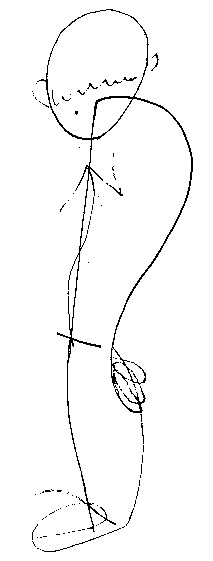
\includegraphics[width=40mm]{./imgs/Image_4.jpg}
 %\end{wrapfigure}

\pagebreak
\thispagestyle{empty}

\begin{vplace}[.50]
\begin{center}
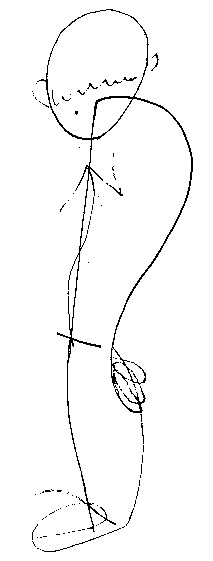
\includegraphics[width=45mm]{./imgs/Image_4.jpg}
\end{center}
\end{vplace}

\pagebreak
\thispagestyle{empty}
\movetooddpage

\letra{S}{e} quiser conhecê"-los depressa, faça"-os brincar. Se quiser ensiná"-los a
viver, deixe os livros de lado. Faça"-os brincar. Se quiser que peguem
gosto pelo trabalho, não os amarre à carteira. Faça"-os brincar. Se
quiser fazer seu trabalho, faça"-os brincar, jogar, brincar.

\bigskip
\bigskip

\letra{S}{e} for professor, foda"-se. Você acredita na eficácia da moral dos salmos
e, para você, a instrução é algo primordial. Se vier trabalhar comigo,
lhe darei os diplomados e ficarei com os iletrados. E conversaremos de
novo no momento da colheita. A instrução é uma ferramenta, maravilhosa,
concordo, indispensável, se quiser. Para nós, o que interessa é quem se
servirá dela.\footnote{Por escrúpulo em relação aos professores, Deligny
  tomou a iniciativa de retirar esse aforismo desde a primeira reedição
  de {\slsc{Semente de crápula}}, pelas Éditions du Scarabée (1960). As
  edições Dunod (1998) conservaram a versão. Optamos por restabelecer o
  aforismo faltante, assim como o fez a publicação nas edições
  L'Arachnéen (2007).}

\bigskip
\bigskip

\letra{N}{ão} seja tão exigente. Eles roubaram peras para comer. Poderiam ter
quebrado os galhos só por prazer. Na escala das más ações, aquelas que
beneficiam realmente soam, no entanto, melhor ao ouvido.

\bigskip
\bigskip

\letra{V}{ocê} não conseguirá nada com a coerção. Poderá, eventualmente, forçá"-los
a ficarem imóveis e em silêncio e, com esse resultado a duras penas
conquistado, você não sairá do lugar.



\letra{S}{e} você cortar a língua que mentiu e a mão que roubou, dentro de alguns
dias será chefe de um pequeno bando de mudos e manetas.



\letra{S}{e} hoje você der um tapa, amanhã terá que dar um soco, já que o tapa não
terá surtido efeito. E depois de amanhã, um golpe com cassetete, e
depois terá que instalar uma câmara de tortura. Acha que estou
exagerando? E quantos reformatórios, no entanto, se enfeitavam com
solitárias, as mais desconfortáveis possível, nas quais se jogava a
criança castigada, privando"-a de comida. Enquanto estava ali, ela
deixava os funcionários em paz, esperando a morte. Ou seja, o cúmulo da
adaptação social.



\letra{V}{ocê} sabe cantar, improvisar uma história de piratas, plantar bananeira,
imitar os gritos dos animais, desenhar nas paredes com um pedaço de
carvão? Então você terá disciplina.

\pagebreak

\letra{N}{as} maiores confusões, você é a calma sorridente. Nas grandes calmarias,
você é o vento.



\letra{D}{ê} um jeito para que eles tenham sempre essa sensação de escolha, fora
da qual não há boa vontade possível.



\letra{O}{} maior mal que você pode lhes causar é prometer e não cumprir. Além
disso, você pagará caro e isso será justiça.



\letra{O}{nde} estão, belos rudes delinquentes, anarquistas, olhos negros, corpos
cálidos dilacerados por cicatrizes? Aqueles que você verá serão glutões
e bajuladores, e desmaiarão se você os vacinar.


\letra{V}{eja} só: você dá uma nota de cem a um fujão e o manda à estação de trem
para comprar uma passagem. Ele volta ofegante e devolve o troco.
``Reeduquei"-o direito?'' Três dias depois, sua cobaia, no meio da noite,
desmonta uma janela e desaparece por um certo tempo. Espero que diga a
si mesmo: ``Parabéns''. Reserve seus experimentos para os ratos brancos.

\pagebreak


\letra{V}{ocê} acredita que o mundo se divide em dois grandes grupos: os que são
honestos e os que não são. Eles lhe dirão: os que são pegos e os que não
são.



\letra{S}{e} você conhece um pouco a aritmética social, você diz a si mesmo que
trinta moleques num dormitório equivalem a dez vezes três amigos, ou
três vezes dez amigos, ou quinze vezes dois amigos. Aqui, infelizmente,
trinta são trinta. Trinta solidões magras, cúmplices e ciumentas.



%\begin{center}
%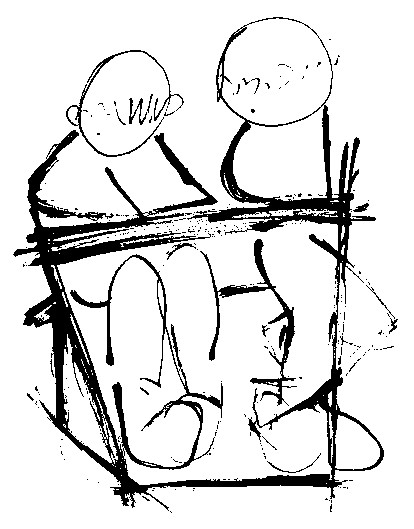
\includegraphics[width=70mm]{./imgs/Image_5.jpg}
%\end{center}

\letra{U}{m} incidente\ldots{} Uma forma de evitá"-lo. Mil formas de desculpá"-lo.



\letra{S}{e} você brincar de polícia, eles brincarão de bandidos. Se você brincar
de Deus, eles brincarão de diabos. Se brincar de carcereiro, eles
brincarão de prisioneiros. Se você for você mesmo, eles ficarão
desconcertados.



\letra{U}{m} olho neles, outro olho no céu. Nos primeiros dias isso dará um pouco
de dor de cabeça.


\pagebreak
\thispagestyle{empty}

\begin{vplace}[.50]
\begin{center}
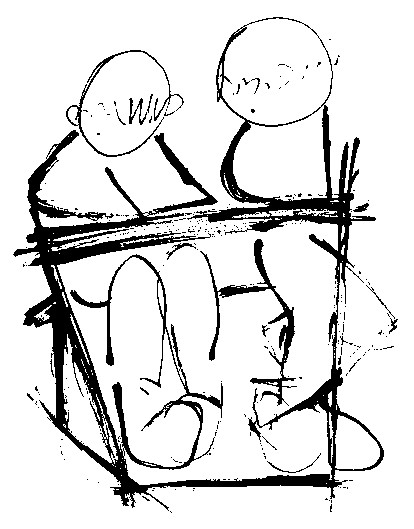
\includegraphics[width=90mm]{./imgs/Image_5.jpg}
\end{center}
\end{vplace}

\pagebreak
\thispagestyle{empty}
\movetooddpage

\letra{A}{quele} que você trata como indiferente e dorminhoco, já reparou com que
destreza e com que vivacidade ele é capaz de afanar um bolo numa
confeitaria cheia de clientes? Ele está vivo. Nem tudo está perdido.



\letra{Q}{uando} H. chegou, todo cheio de qualidades, você se perguntou: ``Mas o
que é que ele vem fazer aqui?'' Agora que o conhece, você diz a si
mesmo: ``O que é que ele poderá fazer lá fora?''



\letra{A}{quele} ali é um autêntico crápula; vem do presídio, amassado e sujo; seu
arquivo está cheio de relatórios detalhados e reincidências. Menos mal,
o trabalho está meio caminho andado. Na montanha, melhor subir que
descer.



\letra{C.}{,} quando chega, se mostra educado, solícito e honesto; é um ator. Será
preciso ensiná"-lo a ser ele mesmo. E, no fim das contas, com a ajuda do
tempo, a se tornar outro.



\letra{T.}{,} que dava chutes nas canelas, agora dá socos na cara. Grande
progresso.

\pagebreak

\letra{L.}{} chega a você da prisão pelo roubo de um coelho que ele dividiu com a
avó. Agradeça à justiça; poderiam ter lhe enviado a avó.



\letra{C}{onheci} um que, quando estava muito ansioso para jogar, chegava a
desmaiar. Ele não tinha coragem de se conter. É o mesmo que tinha jogado
um machado na mãe quando ela recusou lhe dar quarenta tostões. Depois de
sair ``melhorado'', quis violar a irmã menor, que não via há muito
tempo.



\letra{O}{ra} pródigo e avarento, ora audacioso e medroso, ora mesquinho e
desinteressado, aquele ali só é ele mesmo quando está dormindo.



\letra{R.}{} já sabe que a vida não é para ele e, com as mãos nos joelhos, vê
passarem as horas.



\letra{N}{unca} se esqueça de olhar se aquele que se nega a andar não tem um prego
no sapato.



\letra{V}{ocê} os coloca contra uma parede: você faz uma marca poucos milímetros
acima de cada cabeça. Espera que tenham crescido. Labor incessante.

\pagebreak
\thispagestyle{empty}

\begin{vplace}[.50]
\begin{center}
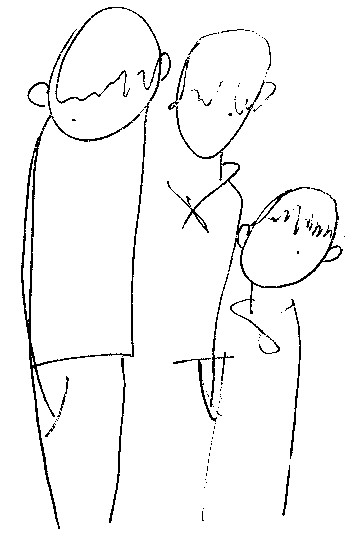
\includegraphics[width=80mm]{./imgs/Image_6.jpg}
\end{center}
\end{vplace}

\pagebreak
\thispagestyle{empty}
\movetooddpage

\letra{E}{steja} presente, sobretudo quando não está ali.



\letra{S}{e} forem roubar morangos, plante morangos no pátio deles.



\letra{C}{apazes} de tudo? É seu esse ``tudo''.



\letra{V}{ocê} os faz cantar cantos que glorificam a beleza do mundo. E o que eles
buscam, olhos baixos, é uma bituca de cigarro solitária.



\letra{V}{ocê} lhes propõe jogos de sua juventude e eles não parecem entender que
esses jogos são mais atrativos que outros.



\letra{E}{les} são quarenta. Você lhes pergunta: ``Quem realmente quer jogar?''
Vinte e cinco levantam a mão.
Você leva todos até a quadra. E são os
outros quinze que jogam.



%\begin{center}
%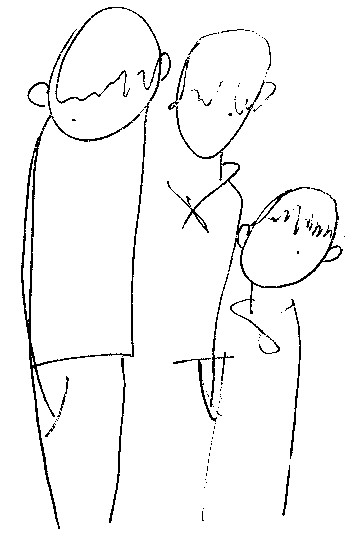
\includegraphics[width=70mm]{./imgs/Image_6.jpg}
%\end{center}
\letra{O}{lhe} aqueles que ficam nos cantos da sala de jogos, rejeitados como
aqueles meninos desengonçados nos ``brinquedos giratórios'' dos parques
de diversões. Será custoso para eles ocuparem seus lugares na
existência.

\pagebreak


\letra{R}{oubaram} quatro torradas. Inquérito rápido. O ladrão é M. Trazem"-no até
você. ``Senhor, eu não farei mais isso, nunca mais, eu juro.'' Ele está
pálido de aflição, chora e retorce as mãos, se entrega e, se fosse mais
forte, teria lavrado seu próprio peito. Você balança a cabeça, atento a
esse debate entre a hereditariedade e a boa vontade nascente. Ele
estende três fatias de pão molhadas em lágrimas: você se emociona. A
outra fatia, a seca, ele a comerá em seguida, bem escondido, à sua
saúde.



\letra{A}{ntes} de se indignar, lembre"-se daquilo que você mesmo era capaz quando
tinha a idade deles.



\letra{V}{ocê} diz a si mesmo: ``Vou substituir o pai e a mãe dele''. Isso não é
razão para você se embebedar todos os dias.



\letra{D}{esconfie:} aquele que se exibe é o que tem vontade de se fazer ver, e,
portanto, de se esconder.



\letra{Q}{uando} tudo funciona, é chegada a hora de começar outra coisa.

\pagebreak
\thispagestyle{empty}

\begin{vplace}[.50]
\begin{center}
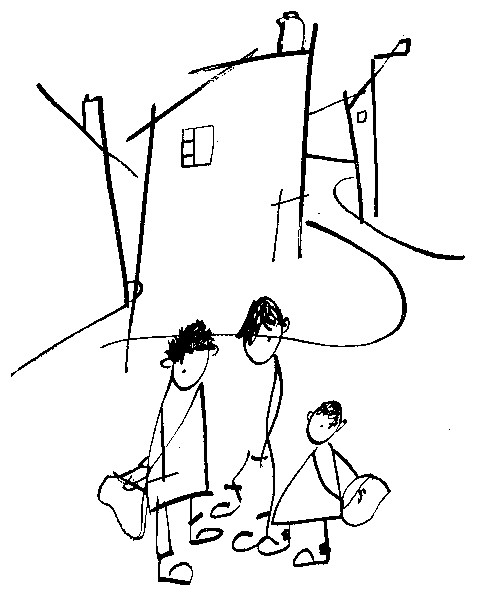
\includegraphics[width=95mm]{./imgs/Image_7.jpg}
\end{center}
\end{vplace}

\bigskip
\bigskip

\pagebreak
\thispagestyle{empty}
\movetooddpage

\letra{E}{sta} noite, eles lhe parecem estranhos e são estranhos uns aos outros; o
ambiente está cinzento: caroços num líquido sujo; tudo falhou. E você
passa a noite com esse peso no coração, totalmente enojado deles. Na
manhã seguinte, encontra"-os frescos e triunfantes, como um doce
bem"-feito.



\letra{Q}{ue} preocupação constante, que espantosa habilidade, que atenção sempre
alerta em evitar o mínimo trabalho! Algo como uma central elétrica que
acionasse um moinho para fumar cigarros.



\letra{S}{e} eles bocejam de boca escancarada enquanto lhe escutam contar uma
história, tome isso, se puder, como uma mostra de confiança.



\letra{N}{ão} se trata de que eles adquiram os hábitos de um adulto, você, mas do
hábito de viver como todo mundo.



\letra{N}{ão} os ensine a serrar se você não souber segurar uma serra; não os
ensine a cantar se você achar chato cantar; não se disponha a ensiná"-los
a viver se você não amar a vida.



%\begin{center}
%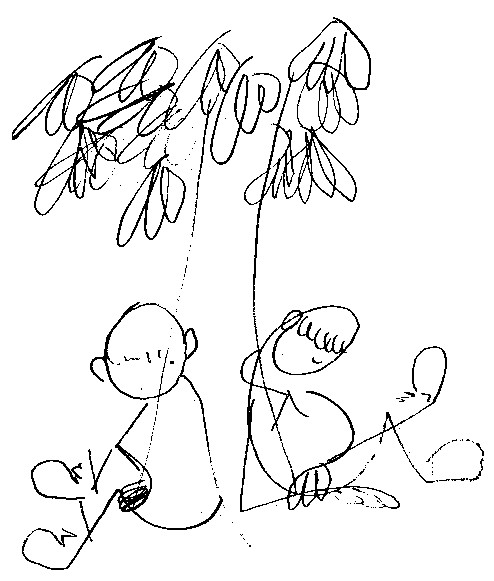
\includegraphics[width=90mm]{./imgs/Image_8.jpg}
%\end{center}
\pagebreak


\letra{M}{aneje} o escotismo com prudência. Eles não precisam olhar os modelos que
você propõe como um sapo olha uma borboleta.



\letra{N}{ão} lhes diga: ``Acha que eu?'' Pode ser que você seja um adulto modelo.
Você certamente já não mais é um modelo de criança. Mas quando se tratar
de ter coragem, você deverá ter por trinta; quando se tratar de ser
teimoso, deverá ser por cinquenta; quando se tratar de rir, precisará de
alegria para cem pequenos enjoados.



\letra{S}{e} no coração de um escoteiro dorme um pequeno cavaleiro, no coração
deles ronca um pequeno operário.



\letra{Q}{uando} lhe falarem de sua abnegação, espero que fique muito surpreso. Se
não ficar, mude de profissão.



\letra{A}{quele} que chora sem parar: faça"-o lavar a sala. Se você tiver pena,
mude de profissão.



\pagebreak
\thispagestyle{empty}

\begin{vplace}[.50]
\begin{center}
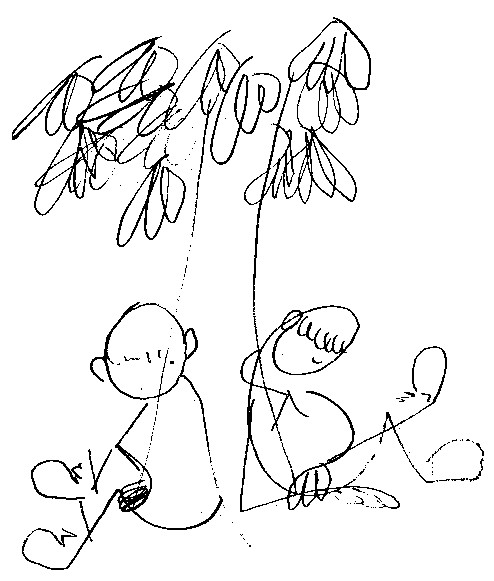
\includegraphics[width=95mm]{./imgs/Image_8.jpg}
\end{center}
\end{vplace}

\pagebreak
\thispagestyle{empty}
\movetooddpage

\letra{N}{ão} se deixe levar até o ponto de dizer: ``Oh! Jean, você fez isso\ldots{}
como você me decepciona.''. Se não for verdade, Jean vai se dar conta
disso. E, se for verdade, você corre o risco de acelerar o ritmo dos
delitos, ainda que seja só para lhe decepcionar. Pois aí está um prazer
do qual Jean foi privado desde que deixou os pais.



\letra{I}{nclinar"-se} demais sobre eles é a melhor posição para receber um chute
no traseiro.



\letra{E}{ra} uma vez um educador que gostava muito deles, mas tanto, que fizeram
dele um grande lenço.



\letra{S}{e} quiser que eles sejam eles mesmos, e você só pode querer isso,
meta"-se no meio deles sem armas e sem couraça, sem castigos nem
recompensas. Se for atacado, pratique, se estritamente necessário, o
jiu"-jitsu, pois tanto essa arte quanto a maneira de usá"-la são fruto do
conhecimento do homem. Digo isso em sentido figurado: está fora de
questão eles lhe atacarem. Se isso acontecer, mude de profissão: é que
você é baixinho demais, tem a cara feia ou os pés chatos.

\pagebreak

\letra{P}{roibir} você de castigá"-los vai lhe obrigar a deixá"-los ocupados.



\letra{D}{epois} da incontinência verbal, o castigo é a arma mais cara aos
corretores de crianças. E o mais triste é que as crianças tomam gosto
por esses vícios de gente grande.



\letra{D}{iga} a si mesmo que a educação começará no dia em que o ambiente estiver
completamente livre do mínimo miasma de ``sanção''. E as mais difíceis
de desinfetar serão, talvez, as crianças.



\letra{O}{s} defeitos deles são como pelos: quanto mais cortamos, mais duros
crescem.



\letra{U}{m} hábito se arranha, um defeito se desbota; não fure o papel.

\pagebreak

\letra{N}{ão} acredite que vai encontrar neles esses defeitos miraculosos que
glorificariam um museu psicológico. Você vai recolher com uma pá a
imensa quantidade de defeitos que se arrastam pelas ruas. Se você se
contentar em colocá"-los numa estufa, cuidadosamente etiquetados e limpos
e espanados todo o mês, eles vão proliferar, crescer e se tornar
monstruosos, como você quer, e a pequena coleção de anormais espantará
os visitantes.



\letra{C}{uidemos} dos delinquentes e castiguemos os tuberculosos. Veremos como
uns se tornam escassos enquanto os outros se multiplicam.



\letra{A}{quele} ali é teimoso, rebelde e preguiçoso. Ele foge. ``Ainda bem: não
havia nada a fazer; os porquinhos vão comê"-lo''. Dois anos depois, ele
vem lhe ver, vestido confortavelmente, dono de uma bicicleta comprada
com suas próprias economias, com um bom trabalho em mãos. Não fique
ofendido. A vida tem muito mais experiência que você.

\pagebreak

%\begin{center}
%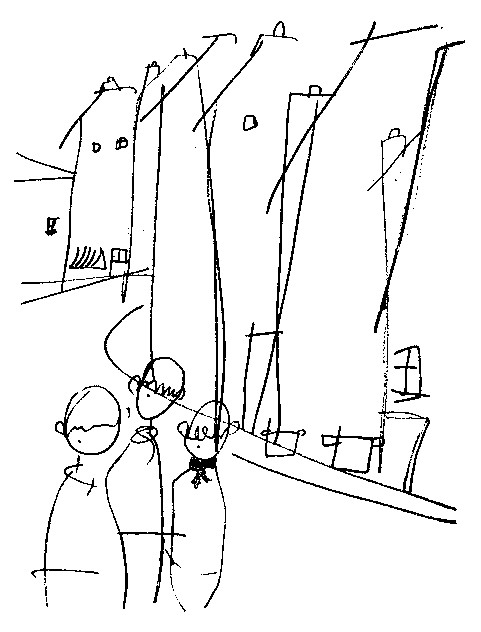
\includegraphics[width=90mm]{./imgs/Image_9.jpg}
%\end{center}

\letra{A}{reje} e limpe: a maldade é um micróbio que prolifera na sombra, na
desordem e na sujeira. A água, o fogo, o ar e a luz: é disso que são
feitos, em nosso ofício, os milagres.



\letra{N}{ão} creia em milagres. Hoje faz sol, o céu está azul e o vento, fresco.
Eles brincam. Ouvindo seus gritos alegres, vendo"-os correrem uns atrás
dos outros e se dispersarem para se reagrupar em bandos amigos, você os
percebe finalmente confiantes e abertos. Bate as mãos para aplaudir essa
confiança finalmente encontrada e para chamá"-los. Quatro deles fugiram.
Prova de que o sol não tem em você e neles o mesmo efeito.



\letra{F}{aça"-os} cantar, rir e dançar; faça"-os correr, suar, saltar. O resto é
questão de prudência e organização.



\letra{N}{ão} investigue as ``historinhas entre eles'' sem segurar firme na escada
pela qual você desceu. Você corre o risco de se asfixiar como no fundo
de um poço.



\pagebreak
\thispagestyle{empty}

\begin{vplace}[.50]
\begin{center}
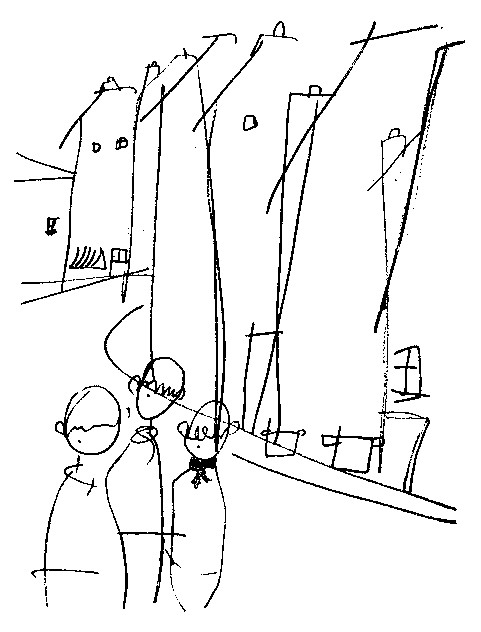
\includegraphics[width=95mm]{./imgs/Image_9.jpg}
\end{center}
\end{vplace}

\pagebreak
\thispagestyle{empty}

\movetooddpage

\letra{J}{ean} pegou a torrada de Paul. Então Paul receberá uma torrada de Jean.
Sim, mas Jean deverá dar a Maurice o torrão de açúcar que Charles o
fizera trocar por um porta"-penas que Henri extorquira de Louis e que ele
recebera de Marcel em troca de um chute no joelho e depois de ameaças
misteriosas, e o tal Marcel havia roubado quatro bolas de gude de Paul
que as tinha pegado emprestadas de Jean. A verdade está no fundo do
poço, mas a corda com a qual você a puxa é tão longa, tão longa, que
quando a verdade chegar à borda você estará muito longe para sequer ver
a cor dos cabelos dela.



\letra{V}{ocê} perceberá que alguns juízes tomam decisões como joalheiros vendem
uma aliança. Um tira a medida do delito tal como o outro tira a medida
do dedo. Tanto um quanto o outro mal se importam com o resto.



\letra{A}{} justiça. Ou: quando o abstrato se torna escrivão.


\pagebreak

\letra{S}{e} estiverem trancafiados tudo o que você pode fazer por eles é
trazer"-lhes três brotinhos de grama fresca, como faz aquela velha que
vem dar uma olhada em seus coelhos na gaiola: bela história, projetos,
músicas de caminhada\ldots{} Mas isso jamais será carne de primeira.


\letra{C}{rie} trutas em água suja, elas pegarão o gosto de lodo. Crie rãs em água
clara, elas pegarão o gosto de truta.



\letra{C}{onstrua} uma fortaleza. Trabalho de escravo ou jogo maravilhoso. Tudo
está na forma de fazer.



\letra{E}{pileptoide,} deprimido, hipomaníaco\ldots{} É isso que o médico olha. Seu
refrão, por sua vez, deve ser: ``Vamos brincar de quê?''



\letra{T.}{} é brutal e teimoso. Não se apresse em tirar suas garras. Talvez elas
sejam suas únicas qualidades.



\letra{P.}{} é mentiroso, H. é insolente, Z. é debochado. E F., que não é nada
disso, o que vamos fazer com ele?

\pagebreak

%\begin{center}
%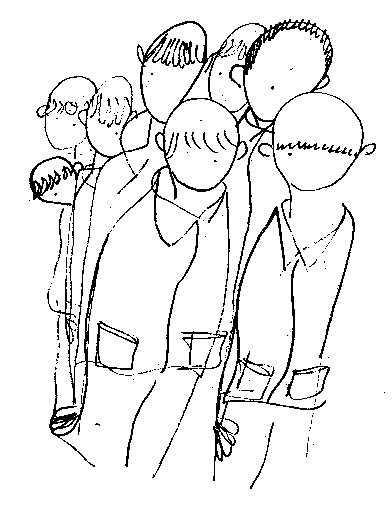
\includegraphics[width=90mm]{./imgs/Image_10.jpg}
%\end{center}

\pagebreak
\thispagestyle{empty}

\begin{vplace}[.50]
\begin{center}
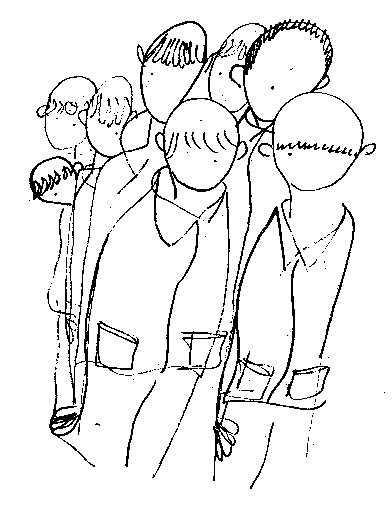
\includegraphics[width=95mm]{./imgs/Image_10.jpg}
\end{center}
\end{vplace}

\pagebreak
\thispagestyle{empty}

\movetooddpage

\letra{H}{á} defeitos úteis, e outros, menos.



\letra{S}{ão} hábeis em perceber seus defeitos de homem, farejando"-os de longe,
como a hiena faz com a carniça, para se empanturrar.



\letra{S}{e} as palavras deles não fossem vãs, você já estaria morto, com os olhos
furados, a língua azul e as entranhas entregues às moscas (se acreditar
neles quando estão com raiva). Se as palavras deles não fossem vãs, eles
seriam corajosos, alegres e honestos, dedicados e conscientes de sua
indignidade (se acreditar neles quando falam com você). Você ainda não
está morto e eles ainda são um pouco crápulas.



\letra{S}{obretudo,} não tente saber o que falam de você entre eles. Eles ficam
com vontade de sair andando quando lhe veem chegar? Eis seu trabalho.



\letra{C}{omo} estão sujos e encardidos, você pensa que talvez seja o caso de
fazer uma grande lavagem da qual eles sairão honestos e corajosos.
Prepare sempre escovas, sabão, água, vento e sol. Então, dia após dia,
você vai habituá"-los a se lavarem a si mesmos.

\pagebreak

\letra{``O}{} vício deles está estampado em seus rostos\ldots{} Olha essas atitudes
dissimuladas\ldots{}''. Escolha o mais perverso da sua equipe, vista"-o como
um pequeno"-burguês, suba com ele num vagão de segunda classe e fale com
ele como se fosse seu filho. Se não lhe disserem ``como seu garotinho é
bem"-comportado\ldots{}'', é porque sua cara não está para conversa.



\letra{A}{quele} que é capaz de suar provavelmente vai se virar. Quanto àquele que
sorri tão gentilmente, nunca faremos dele uma prostituta?



\letra{A}{lguns} estão na beira da honestidade como um convalescente está na beira
da planície: seu quarto cheira à doença, mas, ali, ele está aconchegado.



\pagebreak

\letra{A}{o} redor de um jardim imenso, onde as crianças brincavam entre a relva
alta e os bosques misteriosos, alguém colocou uma barreira. O primeiro
menino que a avistou chamou os outros que, interrompendo o jogo, vieram
olhar, através das barras, o resto de um mundo para o qual eles não
ligavam muito na véspera. E o mistério e o prazer, agora inacessíveis,
passaram ao jardim vizinho. Dito de outro modo: evite as ``interdições''
sob pena de ver seu bando se precipitar e atravessar com prazer as novas
barreiras. 


\letra{D}{esajeitados} no jogo como as corujas na luz. Rancorosos, birrentos,
trapaceiros, mesquinhos e avarentos com o próprio fôlego. De resto, os
melhores filhos do mundo. Preferem mascar fumo e cuspir entre os pés\ldots{}


\letra{D}{esconfie} das soluções imediatas: não adianta nada ligar uma lamparina
de gás na corrente elétrica.


%\begin{center}
%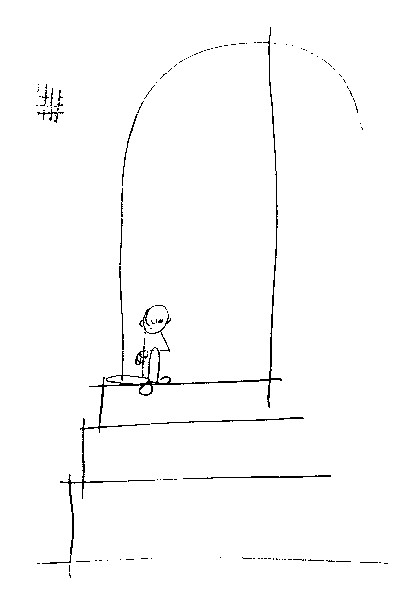
\includegraphics[width=80mm]{./imgs/Image_11.jpg}
%\end{center}

\pagebreak


\letra{E}{les} estão intoxicados por quinze anos de vida num ambiente imundo? Não
têm nenhum gosto por aquilo que é sadio, honesto, humano? Seu trabalho é
justamente o de tornar"-lhes assimilável aquilo de que eles se desviam,
de saber apresentar"-lhes aquilo de que necessitam e de que não gostam
muito: esforço cotidiano, jogos de regras, luz natural, água fresca,
grandes e alegres tapas nas costas dos leais companheiros.



\letra{V}{ocê} aprenderá que roubar habilidosamente está ao alcance do mais besta.



\letra{V}{ocê} reconhecerá entre eles a ostra, a carpa, o boi, a hiena e o cavalo.
Você se irritaria contra uma ostra?



\letra{P}{oupe} suas raivas para os momentos de solidão e, depois, cuidadosamente,
transforme"-as em energia.



\letra{O}{s} pais. Eles demoraram quinze anos e nove meses para fazer de seu filho
o que ele é, e gostariam que, em três semanas, você fizesse dele uma
criança modelo.



\pagebreak
\thispagestyle{empty}

\begin{vplace}[.50]
\begin{center}
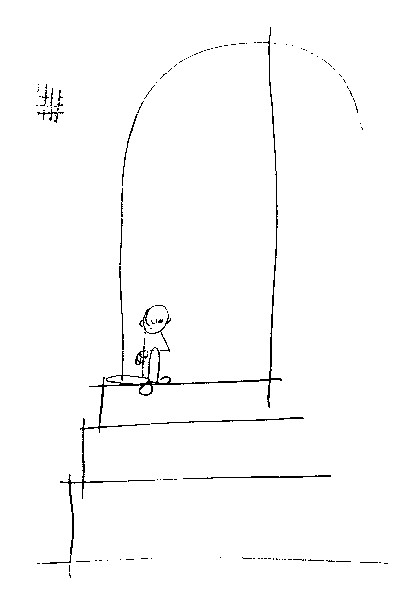
\includegraphics[width=95mm]{./imgs/Image_11.jpg}
\end{center}
\end{vplace}

\pagebreak
\thispagestyle{empty}

\movetooddpage

\letra{S}{e} esses poucos que você terá ``melhorado'', uma vez fora, comportam"-se
mal, você vai pensar, que é o resto do mundo que precisa ser reeducado.
O que não é algo mal pensado. Tarefa à qual outros além de você, e que
eram Deuses, fracassaram em renunciar.



\letra{M}{antenha"-os} vivos. Se a vida para eles é roubar, provocar, destruir,
procure simplesmente para esses verbos os objetos diretos ou indiretos
que farão sua força, imperceptivelmente, derivar para atos louváveis e
úteis.



\letra{M}{eu} primeiro é obediente. Meu segundo é obediente. Meu terceiro é
obediente. Meu quarto é perverso. E meu todo é um belo bando de
trombadinhas.



\letra{E}{le} tem medo dos cães. Tem horror à chuva. Tem pavor ao vento. Sempre
está com frio e fica inquieto quando a comida atrasa cinco minutos. É um
pequeno vagabundo.



\letra{Q}{ue} a sua simpatia por aqueles que, dentre eles, se pareçam com você,
não lhe impeça de compreender os outros.

\pagebreak

\letra{V}{ocê} perde dinheiro. T. encontra dois francos e os guarda. V. encontra
cinco francos e lhe devolve. E eu digo que você terá problemas com V.



\letra{N}{ão} acredite que aquele que rouba de um para dar para os outros está
perto da ``saída''. Se você se misturar com a estética e a moral pura,
será um perigoso egoísta e não está fazendo o seu trabalho.



\letra{Q}{ue} sejam ``como todo mundo'' -- e Deus sabe como é feio o mundo -- aí
está, aí está seu ideal.



\letra{E}{les} vão lhe surpreender: apesar de tudo, bem mais próximos de Pasteur
do que da ostra.



\letra{N}{ão} os largue antes que tenham tirado tudo de bom que poderiam do
ambiente que você criou. Mas quando estiverem bastante confortáveis,
tenha pressa para se separar deles. Para ter um exemplo a dar para os
outros, você se arrisca a deixar apodrecer os mais belos frutos da sua
colheita.




\pagebreak
\thispagestyle{empty}

\begin{vplace}[.50]
\begin{center}
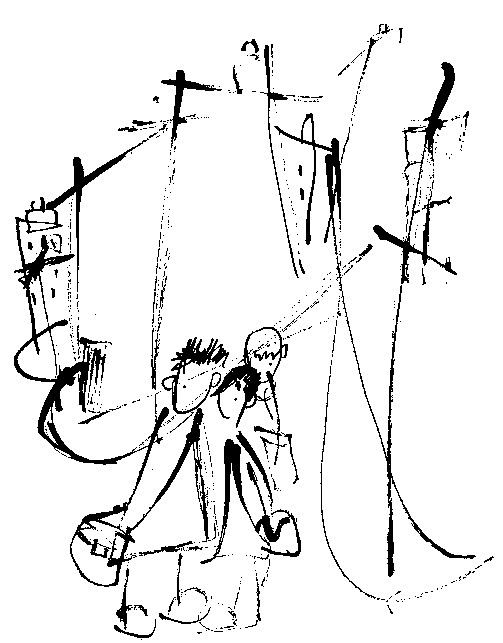
\includegraphics[width=95mm]{./imgs/Image_12.jpg}
\end{center}
\end{vplace}

\pagebreak
\thispagestyle{empty}

\movetooddpage


\letra{P}{ara} lhe consolar. Se você for bem"-sucedido, será mais forte que a
estupidez.



\letra{E}{ra} uma vez um burro, adulto há alguns anos e mestre"-escola
profissional, que batia constantemente nos jovens cordeiros porque suas
orelhas não cresciam rápido o suficiente. Ao seu lado, um velho gerânio
ensinava às jovens violetas como elas deveriam enrubescer. Seguindo o
mesmo trabalho, um velho melro ensinava a duas jovens corujas os
segredos para cantar bem. E esse centro de reeducação era célebre no
mundo inteiro pela excelência de seus métodos, mas não pela eficácia dos
resultados obtidos.



\letra{E}{ra} uma vez um coração de criança povoado de boas intenções, vivas,
discretas e um pouco disformes, como um povoado de anões numa floresta
antiga. Um adulto que passou entoava com a voz grave bons conselhos e
capítulos de moral. Só de ouvir seus nomes arrotados por aquela voz
sonora, todos os anõezinhos morreram de medo. Adultos, sejam menos
barulhentos.


\pagebreak

\letra{E}{spere} o grande cansaço que te chegará, numa noite, junto com a ânsia de
resfolegar, como os cavalos, junto com o desejo de andar na direção do
horizonte até a região das crianças sãs, nobres e harmoniosas, gordinhas
e bronzeadas pelo sol. No dia seguinte, você estará no trabalho uma hora
mais cedo que de costume, como um modo de se desculpar.



\letra{U}{ma} vaca pariu um bezerro de cinco patas. O fazendeiro, toda vez que
passava pelo estábulo, dava quatro ou cinco pauladas na pata extra. A
fazendeira queria mandar o bezerro ao catecismo, para que aprendesse que
ter uma pata a mais era um defeito muito feio. A filha mais velha trazia
suas amigas que explodiam de rir ou faziam cara de nojo. Assim fazem
zigue --- zigue --- zá as casas de educação!



\letra{O}{} pai dele já passou oito anos na prisão; a mãe, dois anos no hospital,
e esse pequeno exigente ainda queria que a sociedade tomasse conta dele.

\pagebreak

\letra{T}{alvez} valesse mais ter, perto das crianças infelizes, velhos
presidiários adornados com o título de educadores em vez de certas
``almas'' de boa vontade. Pois, se uns podem afastar o vício, os outros
podem afastar a vida honesta.



\letra{V}{ivem} nove em dois cômodos. O pai está sempre doente e a mãe sempre
esperando outro irmãozinho. O mais velho está detido por mendigar. Ele
lhe foi confiado. Você lhe dá um sermão. Você também poderia oferecer ao
pai luvas de pele de um animal raro e, à mãe, um alicate de marfim.



\letra{E}{ra} uma vez uma sardinhazinha que não sabia nadar. Colocaram"-na dentro
de uma lata, bem apertada, entre outras duas. Com muito cuidado,
adicionou"-se um pouco de azeite. Como estava feliz a sardinhazinha! Ela
envelheceu três anos. Abriram a lata. Mas ninguém nunca mais tentou
fazê"-la nadar. Pois se tratava de uma sardinhazinha e não de uma criança
delinquente.



\pagebreak

\letra{U}{ma} nação que tolera as favelas, os esgotos a céu aberto, as salas de
aula superlotadas e que ousa castigar os jovens delinquentes, me faz
pensar naquela velha bêbada que vomitava sobre seus filhos durante toda
a semana e que esbofeteou o menorzinho, sem querer, num domingo, porque
ele tinha babado em seu avental.



%\begin{center}
%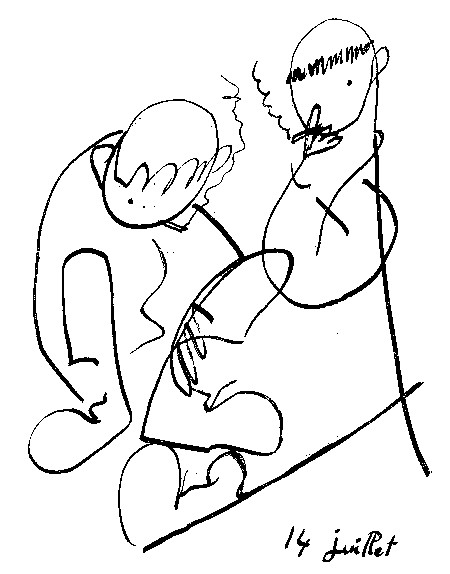
\includegraphics[width=90mm]{./imgs/Image_13.jpg}
%\end{center}

\letra{H}{á} os heredo"-tuberculosos, os heredo"-alcóolatras e os heredo"-infelizes.




\letra{H}{á} três fios que deveriam ser tecidos juntos: o individual, o familiar,
o social. Mas o familiar está um pouco podre, o social está cheio de
nós. Então, tecemos somente o individual. E nos surpreendemos de nada
mais ter feito do que um trabalho de costura, artificial e frágil.



\letra{A}{lguns} dos que fazem esse nosso trabalho creem em Deus; os outros têm fé
nas pessoas.



\pagebreak
\thispagestyle{empty}

\begin{vplace}[.50]
\begin{center}
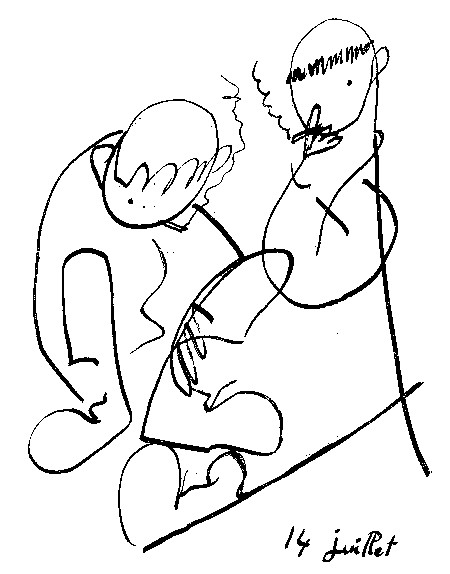
\includegraphics[width=95mm]{./imgs/Image_13.jpg}
\end{center}
\end{vplace}

\pagebreak
\thispagestyle{empty}


\movetooddpage


\letra{Q}{uando} você tiver passado trinta anos da sua vida aperfeiçoando sutis
métodos psico"-pediátricos, médico"-pedagógicos, psicanalo"-pedotécnicos,
na véspera da aposentadoria você pegará uma boa banana de dinamites e,
discretamente, explodirá alguns quarteirões numa favela. Num segundo,
você terá feito mais trabalho do que em trinta anos.

\bigskip
\bigskip

\letra{S}{e} por tão pouco você está desenganado da profissão, não suba em nosso
barco, porque nosso combustível é o fracasso cotidiano, nossas velas se
inflam de zombarias e trabalhamos duro para trazer ao porto uns arenques
muito pequenos, quando tínhamos partido para pescar a baleia.

\bigskip
\bigskip

\letra{É}{} um ofício de crianças, é um ofício de apóstolo, um ofício de
ajustador, ou melhor, de passadeira. E as pregas estão grudadas no corpo
e no espírito das crianças, sobre as quais pesou, com toda sua massa
inerte, uma sociedade de adultos bastante indiferentes.

\pagebreak
\thispagestyle{empty}
\movetooddpage
\thispagestyle{empty}
\setcounter{footnote}{0}
\begin{vplace}[0.25]


{\large\Formular{
\noindent{}Semente de crápula ou\\ o charlatão de boa vontade.\\ Autocrítica de um educador\footnote{Prefácio escrito para a reedição de 1955, não publicado à época.}
}}
\end{vplace}

\pagebreak
\thispagestyle{empty}

\movetooddpage

``Proudhon possui uma inclinação natural para a dialética. Mas, como
nunca compreendeu a verdadeira dialética científica, não foi além dos
sofismas. Na verdade, isso se explica pelo seu ponto de vista
pequeno"-burguês. O pequeno"-burguês constitui"-se de um ``por uma parte''
e de um ``por outra parte''\ldots{} É a contradição personificada. Se, como
Proudhon, ele é uma pessoa de espírito, logo saberá manipular suas
próprias contradições e convertê"-las, segundo as circunstâncias, em
paradoxos evidentes, espetaculares, ora escandalosos, ora brilhantes.
Charlatanismo científico e arranjos políticos são elementos inseparáveis
de semelhante ponto de vista.''

Karl Marx

Ninguém gosta muito de ser pego de surpresa à luz de uma explicação
clara.

Escrevi \emph{Semente de crápula} por volta de 1943. As 136 pequenas
fórmulas foram editadas em 1945. Elas me valeram a simpatia de
educadores próximos e distantes.

Agora, em 1955, uma semana após outra, um pedido chega: dois
\emph{Semente de crápula} aqui, dois \emph{Semente de crápula}
acolá\ldots{} Ora, não há mais \emph{Semente de crápula}. Deve"-se
reeditá"-lo?

Por doze anos, trabalhei. Meu ofício de educador e eu não nos separamos.
A mensagem disparatada de 1943, com suas facetas talhadas em paradoxos,
me irritaria se eu a lesse vinda de um outro. Mas, já que ela ainda
flutua e que, aqui e acolá, jovens educadores ainda querem lê"-la, por
que não retomá"-la, corrigi"-la, a fim de encurtar um dia a estrada
daqueles que querem sair dos repugnantes redemoinhos ideológicos em que
estão presos, primeiramente, aqueles e aquelas cuja tarefa cotidiana
consiste em cuidar de crianças que não nasceram deles.

``Pequeno"-burguês\ldots{}'', eis"-me entregue ao meu lugar (gostaria de poder
escrever ``meu lugar de então'') eu, o educador que se queria, ainda
assim, revolucionário.

Pequeno"-burguês\ldots{} A tribo é numerosa e muito diversa. Pequeno"-burguês
de origem? Por acaso sofri por ser um explorado? Nunca: sempre tive a
sensação de ser um privilegiado. Órfão de guerra, sim, mas órfão de
oficial, e o bairro onde cresci, em Lambersart, perto de Lille, era tão
pequeno"-burguês quanto um bairro pode ser. Ele era assim: \emph{villas},
autênticas \emph{villas}-pequenos"-castelos em cada um dos lados de uma
avenida vizinha de um hipódromo: pode"-se dizer que aquela avenida era a
espinha, a coluna vertebral do lugar. Quem vivia ali dentro? Não faço
ideia: nunca vi, com meus próprios olhos, nada entrar nem sair dali.
Havia árvores que conhecia bem e que eram minha única companhia quando
pegava aquela avenida. Agora, quando vejo tudo aquilo com mais
distância, sei que havia um castelo, uma espécie de castelo, que se
chamava \emph{crépi} {[}reboco{]}, e eu achava que era seu nome de
construção, castelo"-reboco, como diríamos castelo"-pontudo.\footnote{A
  palavra \emph{crépi} se traduz por ``reboco''; \emph{chapeau"-pointu} é
  o tipo de chapéu com a forma pontiaguda. \emph{Chapeau} e
  \emph{chateaux} em Francês soam de modo parecido. Em seguida,
  \emph{crépi} aparece como nome próprio, e, portanto, é a essa confusão
  que o autor se refere ao ouvir a palavra à época.} Na verdade, Crépi
era o sobrenome de um grande empresário têxtil, e tudo parecia indicar
que aquele imponente castelo, de tão safado, havia procriado e gerado
uma centena de \emph{villas}-castelãs, algumas retorcidas, tortas como
solteironas que andam cheias de frescura; as outras, bem burguesas,
fartas, limpas e satisfeitas em seu parque conservado, habitadas por
algum chefe ou subchefe ou notável colaborador; portanto, uma avenida
muito longa composta por esse enxame de \emph{villas} provenientes do
castelo, mas as últimas delas não eram mais do que casas com uma pequena
escadaria ou pequena torre ou um não"-sei"-quê na fachada ou na parte de
trás que lhes permitia aparecer ao longo dessa avenida do Hipódromo, à
espera de quê? de que um dia o castelo"-reboco passasse lentamente diante
delas?

Num extremo da avenida, um canal, o Deûle, e suas barcas amigas; no
outro, um bom e velho prostíbulo, que deve ter sido uma fazenda: um
bordel; à frente, os campos; aqui, ali, nas árvores, alguns ``castelos''
ainda, mas esses não alinhados, colocados ali, em qualquer canto, e uma
estrada pavimentada que insistia em passar com um bonde que sacudia em
todas essas curvas: suas rodas mordiam o trilho, seu mastro pulava: um
bonde não foi feito para passar por um caminho que deveria ser traçado
por gaivotas preocupadas em voar ao redor da propriedade privada, em dar
voltas, em não morder, em passar por onde podiam, por onde têm permissão
de passar: caminho de costume: deve"-se respeitar os costumes.
Frequentemente acontecia de o bonde descarrilar, nervoso, sobrecarregado
por essas complicações, por essas reviravoltas, enlouquecido por essas
afetações, por esses gracejos que o obrigavam a fazer. Ele descarrilava.
Pouco importa: ele estava no fim de seu trajeto: deveria ir até a igreja
-- para que isso? Ele estava sempre mais ou menos vazio, corria, a
marcha engatada na velocidade mais alta, tomado pelo mal das
tempestades, balançava trinta vezes atrás e na frente pelo labirinto de
curvas entre os castelos secretos e parava no ``Canon d'Or'' para fazer
seu serviço, embarcar seu carregamento de uma brava gente, pessoas
recém"-saídas de suas casas de tijolos: avenidas, ruas de casinhas de
tijolos todas iguais, construídas a cada estação do ano: era nessas
casas que viviam os empregados.

Todos ``empregados'', o bonde cheio, as ruas cheias; um bairro, uma
cidade de ``empregados''. Eles tinham a sensação de serem explorados?
Privilegiados, é isso o que eram. Havia muitos empregados de banco, e,
entre os empregados de banco, havia alguns que eram do Banco da França:
privilegiados em relação àqueles que estavam nos pequenos bancos; e os
empregados dos pequenos bancos? Privilegiados em relação àqueles que não
tinham emprego algum ou em relação ao pessoal uniformizado, um
rapaz\footnote{No original \emph{garçon}, que significa menino, rapaz e
  também empregado que presta vários tipos de pequenos serviços.} disso
ou daquilo: ``rapaz'', com cinquenta anos? Privilegiados esses
``rapazes'', pois, em sua maior parte, eram mutilados de guerra: a
mutilação, mesmo a da guerra, era um privilégio? Em relação aos mortos,
aos moribundos, evidentemente eram privilegiados, e o brilho do
privilégio podia ser lido em muitos dos rostos: o bonde lotado voltava
para a cidade pela rua Royale: estritamente verdade.

Eu era, então, órfão e privilegiado, duplamente, triplamente
privilegiado, já que: meu pai morrera na guerra, mas ele morreu oficial:
pequena pensão; ele tinha metido na minha cabeça (ele, ou minha mãe, ou
os dois) o que era preciso para passar no exame das bolsas de estudo:
bolsista; aluno do liceu:\footnote{O liceu era e continua sendo a
  instituição escolar francesa de educação secundária. Na época de
  Deligny, este nível de ensino não era obrigatório.} privilegiado em
relação aos do primário e aos aprendizes.

Privilegiado. Não há dúvida.

Privilegiado, agarre"-se aos seus privilégios, como um acrobata nauseado
ao seu trapézio.

Os operários me pareciam sérios, e cheiravam como homens de uma outra
raça: eles tinham, no bonde, uma presença desajeitada e rude. Macacões
de trabalho, sapatos, suas roupas, suas ferramentas: sobre a plataforma
cheia de seres de pele pálida, estavam entorpecidos, muitas vezes
pensativos e, na hora de descer, se cumprimentavam com um sinal de
cabeça: no meio dessa gente, eles deviam ter medo de seu sotaque, mas eu
via ali um desdém involuntário, o desejo de não fazer ouvir suas vozes
pelos sujeitos ignóbeis que pareciam se conhecer todos entre si. Aliás,
os operários raramente pegavam o bonde, eles iam a pé, e preferiam a rua
Saint"-André à rua Royale, paralela e mais movimentada, ou a esplanada,
ao longo do canal, ou ainda as muralhas, de bicicleta.

O bonde era um privilégio que me deixava tão desconfortável quanto os
outros privilégios que eu devia suportar: órfão, inteligente, aluno do
liceu etc. ``Pequeno"-burguês'', abandone a tribo! É bem isso o que
tentei fazer, mas imagine só! a tribo, nós a temos na cabeça: e, no
entanto, fui procurar trabalho bem longe, não na direção dessas
distâncias geográficas que só me atiçaram por meio de uma imaginação
muito conscientemente gratuita, mas em pleno asilo de alienados. Um
asilo, é muito longe, é uma ilha.

Antes, quando tinha vinte anos, já havia tentado deixar a tribo. Havia
me filiado ao Partido comunista: um local vermelho, rua de Paris. Um
homem estava ali, constantemente: um membro permanente? Para mim, ele
era como o guardião de uma tradição. Era melhor não se fazer de bobo
naquele lugar. Ele e nós, não pesávamos o mesmo peso. Nós, porque éramos
quatro ou cinco estudantes usando a mesma insígnia. Ele e nós não
tínhamos a mesma densidade: tratávamos de estar à altura quando íamos
pegar os folhetos ou os cartazes para distribuir.

Os cartazes. Ali estavam, uma centena, dobrados em cima de uma mesa do
local, carcomida: havia uma tapeçaria rosa empoeirada pelo pó de gesso
que saía por entre os rasgos: parecia as bochechas maquiadas de uma
velha: os cartazes, eu devia pensar que com um cartaz (mas qual?, quais
teriam sido sua cor e seu desenho e suas palavras? Não sabia), um
determinado cartaz que o Partido deveria ter achado, que com esse cartaz
colado por toda parte, a cidade, algumas horas mais tarde, teria entrado
em comoção, todo mundo em marcha, todo mundo exceto alguns medrosos, e,
esse cartaz, não o arrancávamos nunca.

Íamos colar nossos cartazes e, uma vez feito o trabalho, voltávamos a
passar na frente deles para vê"-los: eram humildes, apesar da violência
das palavras de ordem e, quanto a mim, não estava seguro de estar no meu
direito de colar aqueles cartazes nos muros: qual era, no fundo, essa
briga que se arrastava tanto? Os comunistas estavam na cidade como um
caroço numa fruta e eu era de carne, não da mesma madeira da que são
feitos os comunistas.

É impossível deixar a sua tribo, ela é muito ampla, está por toda parte.
Está na luz acima do canal, sobre o canal. Homens e mulheres se cansam
nas barcas ou no caminho, para puxá"-las, os braços balançando, um passo
atrás do outro, curvados para baixo: uma mulher com cabelos grisalhos,
longos, que pendem, uma mulher com cabelos grisalhos que puxa sozinha
uma barca. Estou com essa mulher ou com a luz que se choca contra o
canal? Trata"-se mesmo de um ``\versal{OU}'': estou com a mulher, eu desço para
puxar com ela porque não se deixa uma velha puxar sozinha, mas não verei
mais a luz; deve"-se escolher: a velha ou a luz; azar!, a luz, escolho a
luz: por acaso um homem ``escolhe'' o ar? Necessita dele.

A tribo está por toda parte: está na imensa biblioteca universitária na
qual homens, um ruivo, um negro alto, um velho, estavam ali para nos
adiantar os livros, para nós, os moleques: homens feitos, que haviam
participado da guerra e não sei quê, tudo o que alguns homens têm que
fazer antes de se tornarem visivelmente feitos e tudo o que tinham que
fazer. Nesse caso, tratava"-se de servir a vocês os livros que vocês
tinham que ler: estavam ali como garçonetes num restaurante, e isso
acabava com qualquer vontade de ler. Usavam camisas cinzas. Um deve ter
recebido um estilhaço de granada na cara, um dia, entre 1914 e 1918;
parecia que ele usava uma máscara desanimada: ele lhe estendia o livro
pedido como um mendigo estende o folheto do horóscopo ou o pacote de
envelopes que ele finge estar vendendo. E era nessa biblioteca que
alguém teria que aprender?

A tribo estava nos bares nos quais todos os que sentiam que sobravam no
mundo se faziam companhia durante todo o dia. A tribo estava na
literatura, outra luz que eu devorava com os olhos: a literatura me
falava de tudo. Estava acima da vida dos homens, como a luz acima do
canal e, ao ter que escolher entre viver ou ler, tínhamos que escolher
ler, já que não sabíamos o que viver.

A tribo estava então por toda parte. Para abandoná"-la, era preciso ir
longe.

Lá. O asilo.\footnote{Manicômio.} 1940. A guerra. 1941. O asilo ao longo
de anos. Havia encontrado um ofício: educador. 1943: escrevo
\emph{Semente de crápula}, o qual, seis anos mais tarde, me proponho
criticar. \emph{Semente de crápula} foi lido por alguns milhares de
educadoras e educadores em busca de seu ofício: cinquenta páginas, todas
nutridas pelo leite da tribo pequeno"-burguesa.

Entretanto, trabalhei muito
neste asilo: havia participado da guerra e de tudo o que um homem deve
fazer para parecer um homem feito. Havia um, entre os grandes
caracteropatas, um entre os cem dos que eu não me separava, que andava,
inclinado para frente, um passo depois do outro; contudo, ele não puxava
nada além de si mesmo, e eu estava com ele, no mesmo caminho de terra,
corredor de asilo; ajudava"-o e via, \versal{AINDA ASSIM}, a plena luz do céu.

Mas a tribo é potente: ela era, no próprio crânio de meu estranho
companheiro, nos seus gestos difíceis e fragmentados de
falso"-trabalhador.

Quando tomei nota das frases de \emph{Semente de crápula}, para quem
anotei? Para ninguém: e isso também era coisa da tribo: uma maneira de
fazer bolhas na luz que banha os canais e os campos e as praias enquanto
o homem, no fundo, fica à sua própria pena.

E partir, como muitos outros tentaram, partir para o Taiti, para o
Evereste ou para os Asilos, partir para deixar sua tribo, isso é deixar
o homem: ainda que se parta para viver com os mais desgraçados, os
tortos, os que babam, os malvados, os mancos: um a mais, um a menos, os
mancos estão pouco se fodendo, ou mais ou menos.

Não se deve abandonar os outros. Não se trata de abandonar sua ampla e
sutil tribo pequeno"-burguesa. Deve"-se estar com esses que trabalham para
convencer de que chegou a hora de mudar de ponto de vista. Deve"-se
dizer. Deve"-se cortar, com os dentes se necessário, as amarras que
prendem suas barracas nos lugares desgastados, em plena fome moral.

Desta vez, pelo menos, sei para quem escrevo: para o leitor de
\emph{Semente de crápula} editado em 1945.

Convido"-os, este ano, para perseguirem nas frases das quais gostaram
naquele momento, o hábil pequeno"-burguês educador, que, manejando como
um malabarista suas próprias contradições, elaborou"-as em paradoxos\ldots{}
et cætera\ldots{} Charlatão de boa vontade.

%\textbf{SUMÁRIO}

%Prefácio de 1960

%Semente de crápula (os 134 aforismos)~

%Prefácio inédito de 1955: Semente de crápula ou o charlatão de boa vontade. Autocrítica de um educador

%Sobre a tradução

\pagebreak
\thispagestyle{empty}
\movetooddpage
\thispagestyle{empty}
\setcounter{footnote}{0}
\begin{vplace}[0.25]


{\large\Formular{
\noindent{}Sobre a tradução\footnote{Parte deste e do texto da contracapa
  foi escrita com base em textos de Sandra Alvarez de Toledo presentes
  nos livros {\slsc{Œuvres}} (L'Arachnéen, 2007) e {\slsc{Permitir, trazar,
    ver}} (\scalebox{.8}{MACBA}, 2009).}
}}
\end{vplace}

\pagebreak
\thispagestyle{empty}

\movetooddpage

Os aforismos de \emph{Semente de crápula. Conselhos aos educadores que
gostariam de cultivá"-la} são o resultado das primeiras tentativas de Deligny.
Ele passa os primeiros 20 anos de atuação profissional entre escolas
especiais, instituições médico"-pedagógicas e hospitais psiquiátricos.
Durante a Segunda Guerra, une operários e membros da Resistência em uma
rede de ajuda mútua, alojada em edifícios destruídos ou abandonados nos
bairros populares. Aproxima, assim, pela prática, educadores diplomados,
de origem pequeno"-burguesa, do meio social dos delinquentes.

\emph{Semente de crápula} foi escrito em 1943 e publicado em 1945, numa
edição que esgota rapidamente.

Por ocasião de um primeiro projeto de reedição em 1955, Deligny redige
um prefácio intitulado ``Semente de crápula ou o charlatão de boa
vontade. Autocrítica de um educador''. Mas a reedição, que só aparece em
1960, é publicada com um outro prefácio no qual o autor vislumbra novo
título para o livro: ``Semente de crápula ou o amador de pipas'' (a
palavra ``amateur'' ressoa também com ``amante''). ``Por volta de 1943, eu
me pus a fazer uma pipa, duas pipas: as fórmulas, formulinhas, cantigas,
charadas, aforismos e paradoxos de \emph{Semente de crápula}.'' Deligny
havia iniciado, uns anos antes da reedição, sua conhecida
tentativa/experimentação/invenção com autistas, que durará até sua morte
em 1996. Deligny acolhe autistas sem intenção de curá"-los, e fala do
autismo sem ser psiquiatra.

O projeto de nossa tradução dos aforismos de Se\emph{mente de crápula}
origina"-se em uma prática. A partir da lógica do amante/amador temos
traduzido textos diversos, de autores consagrados a desconhecidos,
dentro de uma ação chamada \emph{Ensaios ignorantes}, que realizamos nos
últimos 9 anos. Juliana conheceu Deligny em 2012 vendo filmes, mapas,
traços, como visitante numa mostra de arte, e ficou, desde então, entre
textos dele no original francês e em tradução espanhola (não havia nada
traduzido em português). Três anos depois, propôs leituras coletivas de
alguns textos de Deligny e foi aí que Luiz se aproximou. Começamos a ler
entre francês e espanhol, vertendo já para nossa língua, de um jeito
\emph{ignorante} (em aliança com Joseph Jacotot): por comparação.
Podemos ler, traduzir, entender e dar a ler. Em 2019, os \emph{Ensaios
ignorantes} foram convidados pela curadoria de Artes Visuais para criar
algo dentro de um festival no complexo hospitalar do Juquery. Decidimos
traduzir os 134 --- Deligny menciona 136 --- aforismos do livro para ocupar o espaço que foi a
recepção da antiga colônia psiquiátrica de Franco da Rocha, e ler os
\emph{conselhos} junto com o público. Havia, então, um objetivo de
migrar o texto do papel para o espaço e para a voz. Nenhum problema:
eram conselhos. Porém, fixar essa tradução em livro seria projeto mais
ousado, pois nossas traduções, até então, vinham desejando soar textos
entre a solidão e o comum de encontros públicos, para agir a partir da
proximidade com as palavras. A n"-1 se animou, pois algo de nossas
posições interessou à editora. Não foi fácil. Deligny nomeou esses
aforismos conselhos, cantigas, charadas, ou seja, algo que se pode dizer
com voz. Ainda que ele tenha sido um escritor impressionante, optamos
por manter ecos dessa voz (advinda de sua prática) nos aforismos em
português. Ele era francês, esperamos que dê para escutar sua língua.
Ele escrevia a partir da prática. Esperamos que se escute aqui algo
da~ação de Deligny. Em sua tentativa de asilo, o agir é também
desprovido de intenção. Nós dois intencionamos nos aproximar do livro,
vigilantes em relação a uma leitura"-tradução"-amadora/amante que o
escutasse de perto. Agora, na língua de chegada, esperamos que nossa
tentativa brote. Agradecemos a Florelle D'Hoest, Maxime Godard e Sandra
Alvarez de Toledo.

\hfill{}\emph{Juliana Jardim e Luiz Pimentel}



\end{document}
